%%%%%%%%%%%%%%%%%%%%%%%%%%%%%%%%%%%%%%%%%%%%%%%%%%%%%%
% A Beamer template for HKUST (GZ)                   %
% Based on THU beamer theme                          %
% Author: Yuxuan HU                                  %
% Date: Aug 2024                                    %
% LPPL Licensed.                                     %
%%%%%%%%%%%%%%%%%%%%%%%%%%%%%%%%%%%%%%%%%%%%%%%%%%%%%%

\documentclass[serif, aspectratio=169]{beamer}
%\documentclass[serif]{beamer}  % for 4:3 ratio
\usepackage[T1]{fontenc} 
\usepackage{fourier} % see "http://faq.ktug.org/wiki/uploads/MathFonts.pdf" for other options
\usepackage{hyperref}
\usepackage{latexsym,amsmath,xcolor,multicol,booktabs,calligra}
\usepackage{graphicx,pstricks,listings,stackengine}
\usepackage{lipsum}

\author{Group7}
\title{ISOM5160 Group Report}
\subtitle{Dataset: amazon\_food\_reviews.csv}
\institute{
   CAO, Xi (21271664)  LI, Heyi () \\
   LIAO, Jingyu (21262106)  LIN, Chuwei (21237955) \\
    YE, Chenwei (21199517) ZHANG, Ziyang (21266920) \\
}
\date{\small \today}
\usepackage{HKUSTstyle}

% defs
\def\cmd#1{\texttt{\color{red}\footnotesize $\backslash$#1}}
\def\env#1{\texttt{\color{blue}\footnotesize #1}}
% set colors
\definecolor{hkustyellow}{RGB}{167, 131, 55}
\definecolor{hkustblue}{RGB}{0, 56, 116}
\definecolor{hkustred}{RGB}{209, 51, 59}


\lstset{
    basicstyle=\ttfamily\small,
    keywordstyle=\bfseries\color{deepblue},
    emphstyle=\ttfamily\color{deepred},    % Custom highlighting style
    stringstyle=\color{deepgreen},
    numbers=left,
    numberstyle=\small\color{halfgray},
    rulesepcolor=\color{red!20!green!20!blue!20},
    frame=shadowbox,
}

%- --- --- --- --- --- --- --- --- --- --- --- --- --- --- --- 
\begin{document}

\begin{frame}
    \titlepage
    \vspace*{-0.6cm}
    \begin{figure}[htpb]
        \begin{center}
            
\includegraphics[keepaspectratio, scale=0.02]{pic/UST.png}
        \end{center}
    \end{figure}
\end{frame}

\begin{frame}    
\tableofcontents[sectionstyle=show,
subsectionstyle=show/shaded/hide,
subsubsectionstyle=show/shaded/hide]
\end{frame}

% Introduction --- --- --- --- --- --- --- --- --- --- --- --- 

\section{Introduction}
\begin{frame}{Background and Motivation}
	\frametitle<presentation>{Background and Motivation}
	\begin{block}{Why to give a presentation:}
		\begin{itemize}
			\item show the main arguments and results of your work
			\item produce interest to read the full paper/report
			\item goal: be educational and also entertaining
		\end{itemize}
	\end{block}
	\begin{block}{Advantages of using \LaTeX ~with the beamer package:}
		\begin{itemize}
			\item very easy if the report is already written in \LaTeX
			\item different themes which are usable in practice
			\item possibility to create handouts using \emph{beamerarticle}
		\end{itemize}
	\end{block}
\end{frame}

\begin{frame}{Research question}

   this is a Research question.

\end{frame}

% Literature Review --- --- --- --- --- --- --- --- --- --- --- 
\section{Literature Review}
\begin{frame}{Research gap}

   this is a Literature gap.

\end{frame}

\begin{frame}{Research question}

   this is a Literature Review.

\end{frame}

% 4. Correlation Between Ratings and Product Descriptions --- ---

\section{Correlation Between Ratings and Product Descriptions}

\begin{frame}{Correlation Between Ratings and Product Descriptions - Overview}
	% \frametitle<presentation>{Overview}

	\footnotesize

	\begin{block}{Steps}
		\begin{enumerate}
			\item Scrape supplementary data from amazon.com
			\item Analyse correlation for both visual \& text information
			\item \textbf{Correlation computation:} We use spearmanr to compute Correlation
		\end{enumerate}
	\end{block}
    
	\begin{block}{Part1. Visual Information Correlation}
		\begin{itemize}
			\item Correlation with the number of sample images
		\end{itemize}
	\end{block}
    
	\begin{block}{Part2. Text Information Correlation}
		\begin{itemize}
			\item Correlation with description length
			\item Correlation with reading ease
			\item Correlation with the marketing tone of the description
            \item Correlation with product description items
            % \emph{beamerarticle}
		\end{itemize}
	\end{block}
    
\end{frame}

\begin{frame}{Supplementary data (Scraped from Amazon's website)}
	
	\vspace{-5pt}
	\begin{figure}
		\centering
			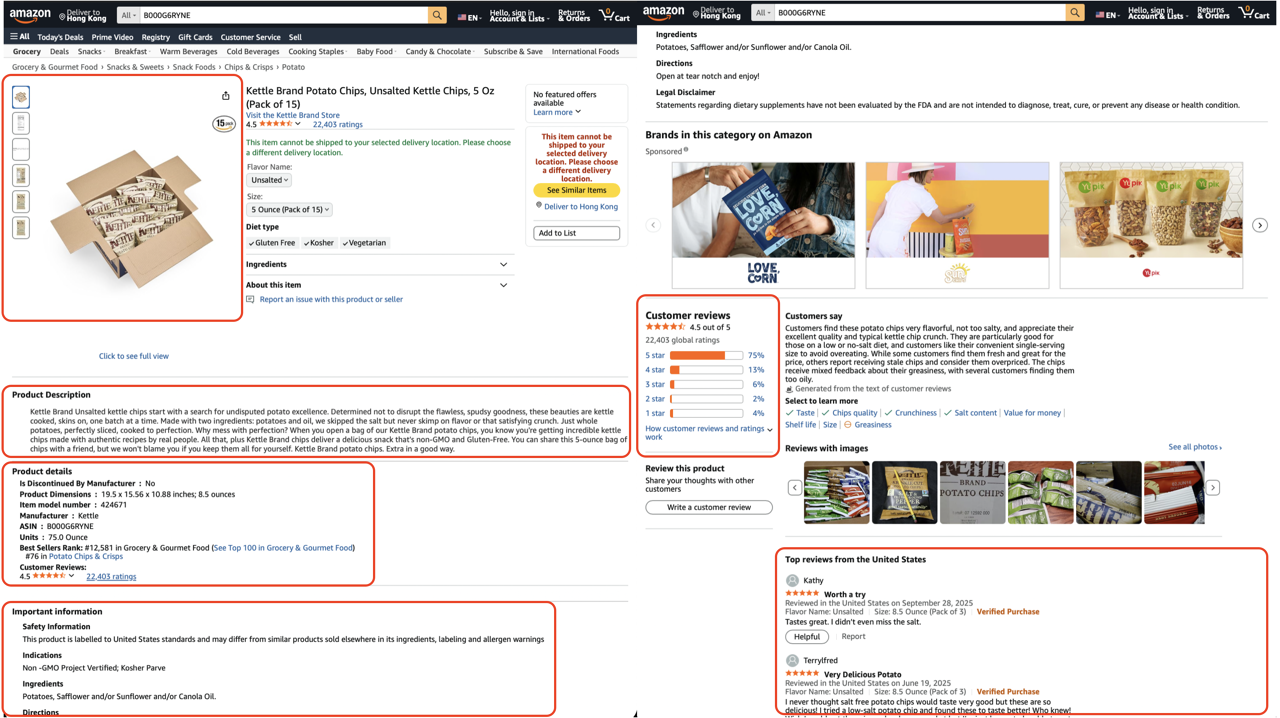
\includegraphics[height=7.3cm]{pic/collected_amazon_data.png}
		% \caption{Logo of the university.}
		% \label{fig:unilogo}
	\end{figure}

\end{frame}

\begin{frame}{Rating features}

	\begin{figure}
		\centering
			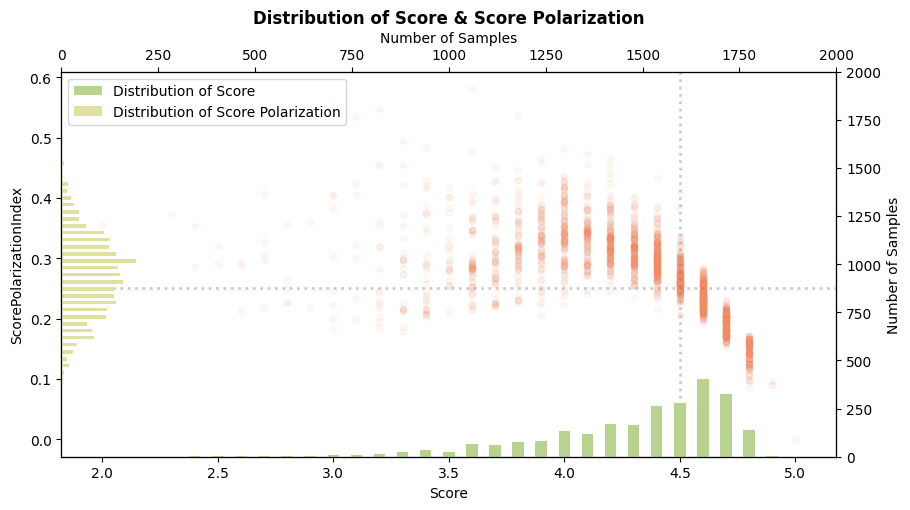
\includegraphics[height=5cm]{pic/score-scatter.png}
		% \caption{Logo of the university.}
		% \label{fig:unilogo}
	\end{figure}

    \begin{enumerate}
        \item \textbf{Mean Score:} The score displayed on the product detail page.
        \item \textbf{Score Polarization:} Indicates whether the ratings for this product are polarized.
        \item \textbf{Standards of Good Score:} Score >= 4.5; Polarization <= 0.25
    \end{enumerate}

\end{frame}
	
\begin{frame}{Correlation with the number of sample images}

	\begin{figure}
		\centering
			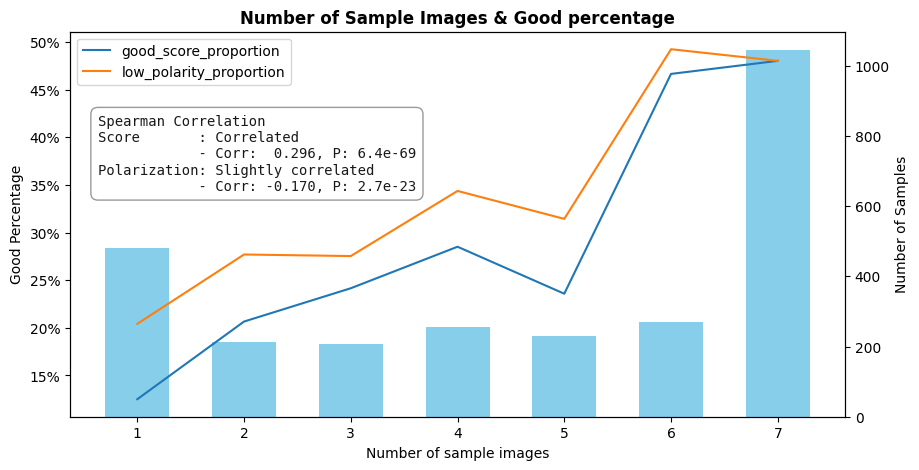
\includegraphics[height=5cm]{pic/corr_n_image.png}
		% \caption{Logo of the university.}
		% \label{fig:unilogo}
	\end{figure}

    \textbf{Conclusion:} The is a \underline{\textbf{positive correlation}} in product ratings and descriptions. The more images included in the description, the greater the likelihood of the product receiving positive reviews.

\end{frame}

\begin{frame}{Correlation with description length}

	\begin{figure}
		\centering
			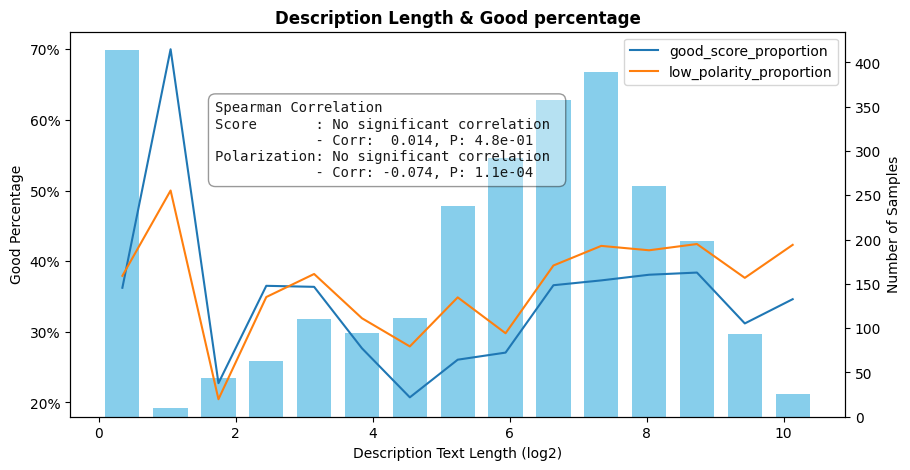
\includegraphics[height=5cm]{pic/corr_len_text.png}
		% \caption{Logo of the university.}
		% \label{fig:unilogo}
	\end{figure}

    \textbf{Conclusion:} There is \underline{\textbf{no significant correlation}} between product ratings and the length of product descriptions.

\end{frame}


\begin{frame}{Correlation with reading ease}

	\begin{figure}[htbp]
	\centering
	\begin{minipage}[t]{0.70\textwidth}
		\vspace{0pt}
		\centering
		\scriptsize
		\begin{tabular}{llrrl}
			\toprule
			ease\_index & compare\_with & corr & p\_value & conclusion \\
			\midrule
				flesch\_reading\_ease & Score & 0.0163 & 0.3863 & No significant correlation \\
				flesch\_reading\_ease & Polarization & -0.0187 & 0.3214 & No significant correlation \\
				flesch\_kincaid\_grade & Score & 0.0123 & 0.5135 & No significant correlation \\
				flesch\_kincaid\_grade & Polarization & -0.0130 & 0.4900 & No significant correlation \\
				gunning\_fog & Score & 0.0066 & 0.7270 & No significant correlation \\
				gunning\_fog & Polarization & -0.0076 & 0.6870 & No significant correlation \\
			\bottomrule
		\end{tabular}
		\normalsize
		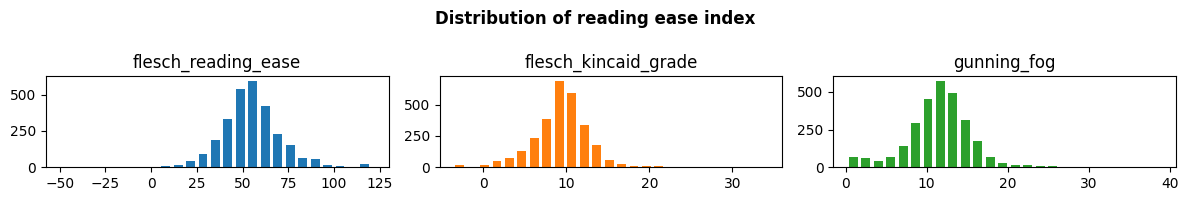
\includegraphics[height=1.86cm]{pic/corr_reading_ease_dist.png}
	\end{minipage}
	\hfill
	\begin{minipage}[t]{0.24\textwidth}
		\vspace{0pt}
		\centering
		\scriptsize
		\begin{itemize}
			\item \textbf{flesch reading ease:} The higher the score, the easier it is to read.
			\item \textbf{flesch kincaid grade:} The required grade level to read; The higher the number, the more difficult the reading level.
			\item \textbf{gunning fog:} Long word ratio; The higher the ratio, the harder it is to understand.
		\end{itemize}
		\normalsize
	\end{minipage}
	\end{figure}

	\textbf{Conclusion:} Product ratings show \underline{\textbf{no significant correlation}} with reading difficulty.

\end{frame}


\begin{frame}{Correlation with the marketing tone of the description}
	\vspace{-16pt}
	\begin{figure}[htbp]
		\centering
		\begin{minipage}[t]{0.50\textwidth}
			\vspace{0pt}
			\centering
			\tiny
			\begin{tabular}{llrrl}
				\toprule
				sentiment\_type & compare\_with & corr & p\_value & conclusion \\
				\midrule
				marketing\_tone\_score & Score & 0.0588 & 0.0007 & No significant correlation \\
				marketing\_tone\_score & Polarization & -0.0469 & 0.0066 & No significant correlation \\
				sentiment\_score & Score & 0.0788 & 0.0000 & No significant correlation \\
				sentiment\_score & Polarization & -0.0568 & 0.0010 & No significant correlation \\
				\bottomrule
			\end{tabular}
			\normalsize
		\end{minipage}
		\hfill
		\begin{minipage}[t]{0.36\textwidth}
			\vspace{0pt}
			\centering
			\begin{figure}
				\centering
					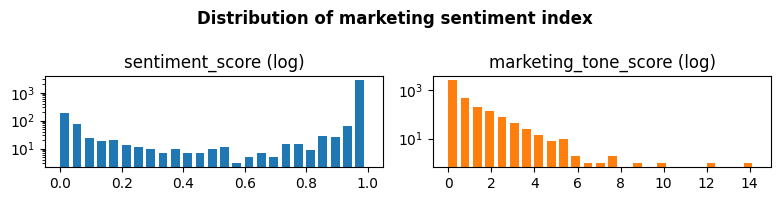
\includegraphics[height=1.45cm]{pic/corr_sentiment_dist.png}
			\end{figure}
		\end{minipage}
	\end{figure}

	\textbf{Types of marketing tone (Measuring Criteria):}
	\footnotesize
	\begin{enumerate}
		\item \textbf{marketing tone score:} The proportion of exaggerated marketing language in product descriptions. The higher the score, the more exaggerated the marketing claims become.
		\item \textbf{sentiment score by language model}: model is distilbert-base-uncased-finetuned-sst-2-english, The higher the score, the more positive the emotion.
	\end{enumerate}
	\normalsize

	\textbf{Conclusion:}
	\footnotesize
	\begin{itemize}
		\item Product ratings \underline{\textbf{show no significant correlation}} with marketing tone/sentiment.
		\item *However, since the metrics used to measure the emotional orientation of product descriptions do not follow a normal distribution, conclusions drawn from this basis may be unreliable.
	\end{itemize}
	\normalsize

\end{frame}


\begin{frame}{Correlation with product description items}
	\vspace{-16pt}
	\begin{figure}[htbp]
		\centering
		\begin{minipage}[t]{0.50\textwidth}
			\vspace{8pt}
			\centering
			\tiny
			\begin{tabular}{llrrl}
				\toprule
				item & compare\_with & corr & p\_value & conclusion \\
				\midrule
				Best Sellers Rank & Score & 0.3809 & 2.9e-116 & Highly correlated \\
				Directions & Score & 0.2211 & 2.12e-38 & Correlated \\
				Item model number & Score & 0.2721 & 4.95e-58 & Correlated \\
				Package Dimensions & Score & -0.2473 & 6.66e-48 & Correlated \\
				Package Dimensions & Polarization & 0.1717 & 1.32e-23 & Slightly correlated \\
				Product Dimensions & Score & 0.2715 & 9.67e-58 & Correlated \\
				Safety Information & Score & 0.1618 & 4.03e-21 & Slightly correlated \\
				\bottomrule
			\end{tabular}
			\normalsize
		\end{minipage}
		\hfill
		\begin{minipage}[t]{0.40\textwidth}
			\vspace{0pt}
			\centering
			\begin{figure}
				\centering
					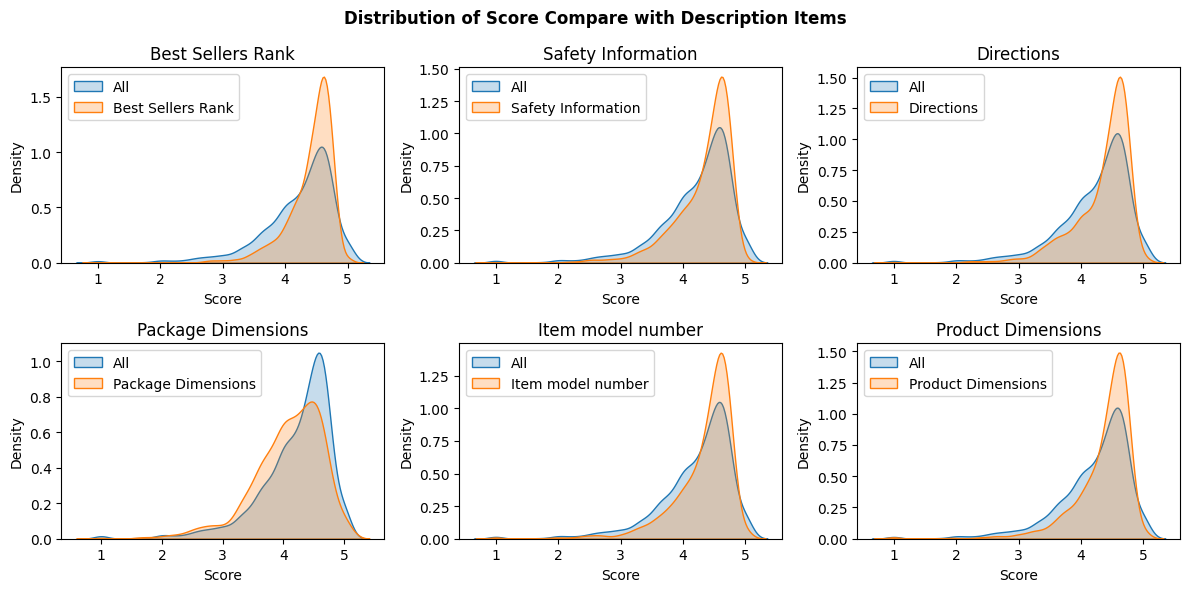
\includegraphics[height=3cm]{pic/corr_desc_item_dist.png}
			\end{figure}
		\end{minipage}
	\end{figure}

	\footnotesize
	\textbf{Products with the following description items might have a better rating:}
	\scriptsize
	\begin{itemize}
		\item \textbf{Best Sellers Rank:} Only high-quality goods carry this label.
		\item \textbf{Item model number \& Product Dimensions:} Products with model numbers may be more formal and reliable.
		\item \textbf{Directions:} Products accompanied by directions may reduce negative reviews caused by users' inability to use or misuse the product.
		\item \textbf{Safety Information:} Products with safety information may reduce negative reviews caused by user allergies.
	\end{itemize}
	\normalsize

	\footnotesize
	\textbf{Products with the following description items might have a lower rating:}
	\scriptsize
	\begin{itemize}
		\item \textbf{Package Dimensions:} May receive negative reviews due to logistics-related issues.
	\end{itemize}
	\normalsize

\end{frame}


% \begin{frame}{Chapter Conclusion}

% 	\begin{block}{For Sellers}
% 		\begin{itemize}
% 			\item Increase the number of product images;
% 			\item Make product descriptions as professional as possible;
% 			\item Provide more detailed safety information and instructions;
% 		\end{itemize}
% 	\end{block}

% 	\begin{block}{For Buyers}
% 		\begin{itemize}
% 			\item Choose products with more pictures;
% 			\item Choose products that appear more professional;
% 			\item Carefully read the product descriptions to avoid potential issues;
% 		\end{itemize}
% 	\end{block}

% \end{frame}






% Methods --- --- --- --- --- --- --- --- --- --- --- 
\section{Methods}
\begin{frame}{Title}
    \begin{itemize}
        \item different themes which are usable in practice
    \end{itemize}
\end{frame}

\begin{frame}
	\frametitle<presentation>{Figures}
	\begin{figure}
		\centering
			
\includegraphics[height=5cm]{pic/UST.png}
		\caption{Logo of the university.}
		\label{fig:unilogo}
	\end{figure}
\end{frame}


% Results --- --- --- --- --- --- --- --- --- --- --- 
\section{Results}
\begin{frame}
    \begin{itemize}
        \item different themes
        \item different themes
        \item different themes
        \item different themes
    \end{itemize}
\end{frame}


% --- Thank you slide ---
\begin{frame}
\begin{center}
{ Thank you for listening !}
\vspace{1cm}

Your Name \\[1em]
@connect.hkust-gz.edu.cn 
\end{center}
\end{frame}

\end{document}